\FloatBarrier
\section{Method of regularised stokeslets} \label{sec:MRS}
\sectionmark{MRS}

When analysing many physical systems, particularly in microscopic biology, it is found that the inertial forces within the fluid are small in comparison to that of the viscous terms. These scenarios occur either where $\mu$ is large or at small length scales where $L$ (the typical scale of the system) is small, such as the flows around cells, microorganisms, or small capillaries \cite{Blake1972AOrganisms, Higdon1979APropulsion, Smith2009MathematicalFluids}.
In these cases, we can take the limit of the Navier-Stokes equation 
\begin{equation}
\label{eq:NavierStokes}
\begin{aligned}
    \rho \left(\dfrac{\partial \mathbf{u}}{\partial t}+(\mathbf{u} \cdot \nabla) \mathbf{u}\right) &= \mathbf{F}-\nabla p+\mu  \Delta \mathbf{u}\\
    \nabla\cdot\mathbf{u} = 0
\end{aligned}
\end{equation}
where $\rho$ is the fluid density, $\mathbf{u}$ is the velocity of the fluid, $\mathbf{F}$ is the external force, $p$ is the pressure and $\mu$ is the fluid viscosity, as $Re=\rho u L/\mu \to 0 $ where $u$ is the magnitude of the fluid velocity $\mathbf{u}$ \cite{Trombley2019BasicFlows}.
In this limit the steady-state Stokes equations in two or three dimensions is obtained as 
\begin{subequations}
\label{eq:StokesFlow}
\begin{align}
    \mu\Delta\boldsymbol{u} &= \nabla p - \boldsymbol{F} \label{eq:StokesFlow1} \\
    \nabla \cdot \boldsymbol{u} &= 0 \label{eq:StokesFlow2}
\end{align}
\end{subequations}
where $\bm{u}$ is the velocity of the fluid, $\bm{F}$ is the external body force, $p$ is the pressure and $\mu$ is the fluid viscosity. We typically also assume a no slip, no penatration boundary condition $\bm{u}(\bm{x},t)=\dot{\bm{x}}$, for all points $\bm{x}$ on the boundary. 

When looking for solutions to the Stokes equation \cref{eq:StokesFlow} there are many different techniques that can use, both numerically and analytically. In this paper will be focusing on the use of the Green's function of Stokes flow $S_{jk}$ called a stokeslet \cite{Pozrikidis1992BoundaryFlow,Hancock1953TheLiquids} or Oseen tensor \cite{Oseen1927NeuereHydrodynamik}. The stokeslet represents a fundamental solution for the velocity of the fluid given that an external force per unit volume $\bm{F}$ acts on the fluid at the origin $\bm{F} = \bm{f_0}\delta(\bm{x})$ \cite{Hancock1953TheLiquids, Batchelor2000AnDynamics}.
Through similar methods to those shown later for deriving the regularised stokeslet Equation, (\cref{eq:regstokeslet2}) it is possible to derive the singular fundamental solutions to the Stokes equations as
\begin{equation}
\label{eq:singularsolutions}
\begin{aligned}
    S_{j k}(\bm{x}, \bm{y}) &= \frac{\delta_{j k}}{r}+\frac{\left(x_{j}-y_{j}\right)\left(x_{k}-y_{k}\right)}{r^{3}} \\
    P_{k}(\bm{x}, \bm{y}) &= \frac{x_{k}-y_{k}}{r^{3}} \\
    T_{ijk}(\bm{x}, \bm{y}) &= \frac{-6\left(x_{i}-y_{i}\right)\left(x_{j}-y_{j}\right)\left(x_{k}-y_{k}\right)}{r^5}
\end{aligned}
\end{equation}
Where $r=|\bm{x}-\bm{y}|$. The pair of tensors $S_{jk}$ and $P_k$ provide the solution to the stokes equation \cref{eq:StokesFlow} with
\begin{equation*}
    \mathbf{u} = (8 \pi \mu)^{-1} \left(S_{1j},S_{2j},S_{3j}\right)f_{0,j}, \quad p = (8 \pi)^{-1} P_k f_{0,j} 
\end{equation*}
where $\bm{f_{0}}$ is the force per unit area exerted by the fluid on the surface, concentrated at the point $\bm{y}$. The final tensor $T_{ijk}$ is known as the stresslet and allows for the stress corresponding the fluid velocity and pressure as $\sigma_{ik}=(8 \pi \mu)^{-1}T_{ijk}$. 

Before 2001 the majority of studies done with stokes flow was done through methods such as slender body theory \cite{Walker2020AFilaments,Johnson1980AnFlow} or the standard boundary element method \cite{Acrivos1975StokesSolution,Pozrikidis1992BoundaryFlow,Tran-Cong1987APropulsion}. Slender body theory applies to only only slender bodies in which the length of the body $l >> 2a$ where $a$ is the radius of the body. While this method allows for the modelling of flagella and cilia has limited applications for more complex geometries. Work done by Youngren and Acrivos \cite{Acrivos1975StokesSolution} which was later review and expanded on by Pozrikidis \cite{Pozrikidis1992BoundaryFlow} shows that the singular stokeslet solution can be formulated into a boundary integral problem where the fluid flow in the domain can be found in terms of an integral over the boundaries of the problem. This lead to the formulation of an Boundary Element Method (BEM) for numerically solving stokes flow problems. While the BEM provides solutions for more complex geometries accurately and efficiently however the need to form a smooth surface mesh and deal with the singular integrals leads to complex force implementation particularly for researchers who are not computational specialists. This problem is eliminated partly by packages such as BEMLIB \cite{BEMLIB} its still requires some computational problem to implement efficiently.

In 2001, Cortez \cite{Cortez2001} proposed the method of regularised stokeslet which was later expanded into into three dimensions in 2005 by Cortez, Fauci and Medovikov \cite{Cortez2005}. The method of regularised stokeslets removes the need to generate a smooth connected mesh as well as the requirement to evaluate singular integrals by replacing the Dirac delta force per-unit-volume with a cutoff function which spreads the force over a finite non zero volume. This allows for stokes flow problem to be solved by simply scattering quadrature points over the surface of the boundary and then evaluating the velocity at the required collocation points.

\subsection{Regularising the stokeslet}

In order to remove the singularities in the stokelet and stresslet solutions, Cortez \cite{Cortez2001} introduced a cutoff function, such that instead of approximating the force at a singular point, it is instead approximated as a sphere centred at the same point. While the radius of the sphere is often infinite, the magnitude of the cutoff function decays rapidly away from the centre with the largest contribution obtained in the close vicinity of the centre of the sphere. A  control parameter $\epsilon$ is introduced to control the rate of decay of the function with its effect shown in \cref{fig:blobfunc}. To obtain similar results to that of the singular solutions, we dictate that $\int_0^\infty \phi^\epsilon(r) r dr=1$ for all values of $\epsilon$. This allows for the preservation of results obtained for the singular kernels for points far away from where the force is exerted, and obtain different non singular results close to the point due to the regularisation error introduced. To retain the singular solution, the condition that as $\epsilon \to 0$ the cutoff function must tend to the Dirac delta function such that we can recover the singular solutions. For simplicity of the paper and the application to a wider range of problems \cite{Olson2013ModelingFormulation}, we will only consider spherically symmetric functions.

\begin{figure}
    \centering
    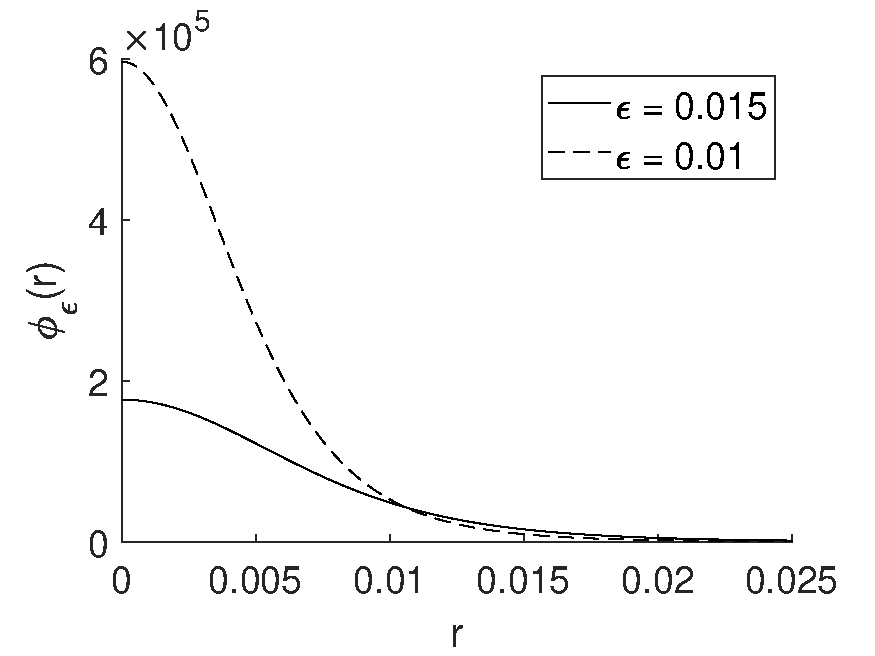
\includegraphics[width=0.5\textwidth]{Images/BlobFunc.pdf}
    \caption{Cutoff function in equation \cref{eq:blobfunc} for several values of $\epsilon$}
    \label{fig:blobfunc}
\end{figure}

\subsubsection{Derivation of the regularised stokeslet}
 By concentrating the force onto a finite area using the cutoff function, rather than a singular point as with the delta function, Cortez proposed to convert the Stokes equations given in \cref{eq:StokesFlow} to a new set of regularised equations,
\begin{subequations}
\label{eq:RegStokesFlow}
\begin{align}
    \mu\Delta\boldsymbol{u} &= \nabla p - \phi^{\epsilon}(\bm{x}-\bm{y})\bm{f_0} \label{eq:RegStokesFlow1} \\
    \nabla \cdot \boldsymbol{u} &= 0 \label{eq:RegStokesFlow2}
\end{align}
\end{subequations}
where $\bm{f}_0$ is the force per unit area as defined in an earlier section.
To simplify notation from this point onwards, we will use the Einstein summation convention where repeated indices are summed over. As with the singular case the regularised stokeslet tensor $S^\epsilon_{ij}(\bm{x},\bm{y})$ is introduced. The regularised stokeslet tensor is the Green's function for the velocity $\mathbf{u}^\epsilon(\bm{x})$ and as such the solution to the regularised Stokes equations \cref{eq:RegStokesFlow} can be written as
\begin{equation}
\label{eq:regvelsol}
    u_i(\bm{x}) = \frac{1}{8\pi\mu}S^\epsilon_{ij}(\bm{x},\bm{y})f_{0,j}
\end{equation}

The pressure and stress tensor associated with this flow can now be written as
\begin{gather}
\label{eq:regpressuresol}
    p(\bm{x}) = \frac{1}{8\pi}P^\epsilon_{j}(\bm{x},\bm{y})f_{0,j}\\
\label{eq:regstresssol}
    \sigma_{ik}(\bm{x}) = \frac{1}{8\pi}T^\epsilon_{ijk}(\bm{x},\bm{y})f_{0,j}
\end{gather}
By substituting these solutions back into \cref{eq:RegStokesFlow1} it is found that the equations must obey the relation,
\begin{equation}
\label{eq:regcondition1}
    \Delta S^\epsilon_{kj}(\bm{x},\bm{y}) = \frac{\partial P^\epsilon_{j}(\bm{x},\bm{y})}{\partial x_k} - 8\pi\delta_{kj}\phi^\epsilon(\bm{x}-\bm{y})
\end{equation}
for all $j=1,2,3$ and $k=1,2,3$ with $\delta_{kj}$ being the Kronecker delta function. The incompressibility condition \cref{eq:RegStokesFlow2} provides a second condition as
\begin{equation}
\label{eq:regcondition2}
    \frac{\partial S^\epsilon_{ij}(\bm{x},\bm{y})}{\partial x_i} = 0
\end{equation}
for all $j=1,2,3$. By taking the derivative of \cref{eq:regcondition1} with respect to $x_k$ to get
\begin{equation*}
    \frac{\partial S^\epsilon_{kj}(\bm{x},\bm{y})}{\partial x_i \partial x_i \partial x_k} = \frac{\partial^2 P^\epsilon_{j}(\bm{x},\bm{y})}{\partial x_k^2} - 8\pi\delta_{kj}\frac{\partial \phi^\epsilon(\bm{x}-\bm{y})}{\partial x_k}
\end{equation*}

Summing over $k$ as per the convention and using \cref{eq:regcondition2} gives
\begin{equation}
\label{eq:regpressureeq}
    \Delta P^\epsilon_{j}(\bm{x},\bm{y}) = 8\pi\frac{\partial \phi^\epsilon(\bm{x}-\bm{y})}{\partial x_j}.
\end{equation}

To solve the regularised Stokes equation, the regularised Laplace's equation \cref{eq:inter1} is introduced which has solution $G^\epsilon$ and the Poisson equation with solution $B^\epsilon$ \cref{eq:inter2}. These equation are linked by the solution to the Laplace equation forming the right hand side of the Poisson equation. This means \cref{eq:inter2} can written as a regularised biharmonic equation $\Delta \Delta B^\epsilon  (\bm{x}-\bm{y}) = \phi^\epsilon(\bm{x}-\bm{y})$. 
\begin{subequations}
\label{eq:intermediate}
\begin{align}
    \Delta G^\epsilon(\bm{x}-\bm{y})  &= \phi^\epsilon(\bm{x}-\bm{y}) \label{eq:inter1} \\
    \Delta B^\epsilon(\bm{x}-\bm{y})  &= G^\epsilon(\bm{x}-\bm{y}) \label{eq:inter2}
\end{align}
\end{subequations}
In this change of variable, we are now working with scalar potentials $G^\epsilon$ and $B^\epsilon$ instead of the pressure and velocity. This allows the pressure tensor, second rank stokeslet and Stress tensor to expressed in terms of these potentials. Combining \cref{eq:inter1,eq:regpressureeq,eq:regcondition1,eq:inter2} the solutions for $P^\epsilon$ and $S_{ij}$ can be expressed in terms of $G^\epsilon$ and $B^\epsilon$,
\begin{equation}
\label{eq:pressuresol}
    P^\epsilon_{j}(\bm{x},\bm{y}) = 8 \pi \frac{\partial G^\epsilon(\bm{x}-\bm{y})}{\partial x_j}
\end{equation}
and
\begin{equation}
\label{eq:regstokeslet1}
    S_{ij}^\epsilon(\bm{x}, \bm{y}) = 8\pi\left[ \frac{\partial^2 B^\epsilon(\bm{x} -\bm{y})}{\partial x_i \partial x_j} - \delta_{ij}  G^\epsilon(\bm{x} -\bm{y})\right]
\end{equation}

Using the definition of the regularised stress tensor 
\begin{equation}
\label{eq:regstress}
    \sigma_{ij}^\epsilon(\bm{x}) = -\delta_{ik}p^\epsilon(\bm{x}) + \mu\left( \frac{\partial u^\epsilon_i}{\partial x_k} + \frac{\partial u^\epsilon_k}{\partial x_i} \right)
\end{equation}
and the definition of velocity in terms of the stokeslet \cref{eq:regvelsol} we find that the stress tensor can be written as 
\begin{equation}
\label{eq:regDoubleLayerSol}
    T^\epsilon_{ijk}(\bm{x},\bm{y}) = -\delta_{ik} P^\epsilon_j(\bm{x},\bm{y}) + \mu\left( \frac{\partial S^\epsilon_{ij}(\bm{x},\bm{y})}{\partial x_k} + \frac{\partial S^\epsilon_{kj}(\bm{x},\bm{y})}{\partial x_i}\right)
\end{equation}

\subsubsection{Specific cutoff function}
For the derivation of the regularised stokeslets and all further numerical analysis, we will use \cref{eq:blobfunc} due to its popularity in external literature and the simplicity of the kernel it generates. Although for more specific problems alternative cutoff functions such as \cref{eq:blobfunc2,eq:blobfunc3} can be used \cite{Olson2013ModelingFormulation,Nguyen2014ReductionFlow,Zhao2019}.
\begin{align}
    \label{eq:blobfunc}\phi^\epsilon(r) &= \dfrac{15 \epsilon^4}{8\pi\left( r^2 +\epsilon^2 \right)^{7/2}} \\
    \label{eq:blobfunc2}\phi^{\epsilon}(r) &= \dfrac{15 \epsilon^{6}\left(5-\frac{2 r^{2}}{\epsilon^{2}}\right)}{16 \pi\left(r^{2}+\epsilon^{2}\right)^{9 / 2}}\\
    \label{eq:blobfunc3}\phi^{\epsilon}(r) &= \dfrac{5 \epsilon^{2}-2 r^{2}}{2 \pi^{3 / 2} \epsilon^{5}} e^{-r^{2} / \epsilon^{2}} 
\end{align}

By solving the Laplace and Poisson equation's for \cref{eq:blobfunc} it is found that
\begin{subequations}
\begin{align}
    G^\varepsilon(\bm{x}-\bm{y}) &= \frac{-2r^2+3\epsilon^2}{8\pi(r^2+\epsilon^2)^{3/2}} + \frac{3}{8\pi\epsilon} \label{eq:G}\\
    B^\varepsilon(\bm{x}-\bm{y}) &= -\frac{\sqrt{\epsilon^2+r^2}}{8\pi} + \frac{r^2}{16\pi\epsilon} + \frac{\epsilon}{8\pi}\label{eq:B}
\end{align}
\end{subequations}
where $r=|\bm{x}-\bm{y}|$. 

Substituting \cref{eq:G,eq:B} into \cref{eq:pressuresol,eq:regstokeslet1,eq:regDoubleLayerSol} to obtain the final kernels which will be used in all further analysis.
\begin{subequations}
\begin{align}
    S_{ij}^\epsilon(\bm{x}, \bm{y}) =& \delta_{ij} \frac{r^2+2\epsilon^2}{\left( r^2 + \epsilon^2 \right)^{3/2}} + \frac{(x_i-y_{i})(x_j-y_{j})}{\left( r^2 + \epsilon^2 \right)^{3/2}}, \label{eq:regstokeslet2} \\
    P_j^\epsilon(\bm{x}, \bm{y}) =& (x_j-y_{j})\frac{2r^2+5\epsilon^2}{(r^2+\epsilon^2)^{5/2}} \text{ and } \label{eq:pressuresol2} \\
    T_{ijk}^\epsilon(\bm{x}, \bm{y}) =& \frac{-6(x_i-y_{i})(x_j-y_{j})(x_k-y_{k})}{(r^2+\epsilon^2)^{5/2}} \label{eq:doublelayer2}\\
    &-\frac{3\epsilon^2[\delta_{jk}(x_i-y_{i}) +\delta_{ik}(x_j-y_{j})+\delta_{ij}(x_k-y_{k})]}{(r^2+\epsilon^2)^{5/2}}. \nonumber
\end{align}
\end{subequations}
It is easily checked that these solutions provide results consistent with those found by the singular solutions, as in the limit $\epsilon \to 0$  the singular solutions stated in \cref{eq:singularsolutions} are obtained.

\subsubsection{Boundary integral equations}
Work done by Pozrikidis \cite{Pozrikidis1992BoundaryFlow} shows that as the Stokes flow equations are elliptic partial differential equations the solution for the entire fluid domain can be represented in terms of a boundary integral over the surface of any bodies in the domain \cite{Stakgold1968Boundary2}. The most common starting point for deriving the Boundary integral equations is that of the Lorentz reciprocal identity which states, for any two non-singular (regular) flows $u$ and $u^\prime$ with stress $\sigma$ and $\sigma^\prime$ respectively, that
\begin{equation*}
    \frac{\partial}{\partial x_k}(u_i^\prime\sigma_{ik} - u_i \sigma^\prime_{ik}) = 0
\end{equation*}
Cortez presents a modified version of the Lorentz reciprocal identity to calculate the boundary integral equation of regularised stokeslets, if we consider the Stokes equations
\begin{equation}
    \label{eq:BIE1}
\begin{aligned}
      \mu\Delta\boldsymbol{u} &= \nabla p \\
      \nabla \cdot \boldsymbol{u} &= 0
\end{aligned}
\end{equation}
and the regularised Stokes equations
\begin{equation}
    \label{eq:BIE2}
\begin{aligned}
      \mu\Delta\boldsymbol{u} &= \nabla p - \phi_{\epsilon}(\bm{x}-\bm{x_0})\bm{f_0} \\
      \nabla \cdot \boldsymbol{u} &= 0
\end{aligned}
\end{equation}
where the solutions are linked through the cutoff function and obtain the same results in the limit as $\epsilon \to 0$. It is assumed that the regularised solution is a flow generated by a point force of strength $\bm{f_0}$ located at a point $\bm{y}$ while the non-regularised solution is absent of all forces. Let $D$ be a rigid body and assume the point $\bm{x}$ is outside of $D$. Then ($\bm{u},p$) must satisfies \cref{eq:BIE1} with
\begin{equation*}
\sigma_{ij}(\bm{x}) = -\delta_{ik}p(\bm{x}) + \mu\left( \frac{\partial u_i}{\partial x_k} + \frac{\partial u_k}{\partial x_i} \right)
\end{equation*}
and ($\bm{u^\epsilon},p$) satisfies \cref{eq:BIE2} with
\begin{equation*}
\sigma^\epsilon_{ij}(\bm{x}) = -\delta_{ik}p^\epsilon(\bm{x}) + \mu\left( \frac{\partial u^\epsilon_i}{\partial x_k} + \frac{\partial u^\epsilon_k}{\partial x_i} \right).
\end{equation*}
We note that $\partial \sigma_{ik}(\bm{x})/ \partial x_k = 0$ and $\partial \sigma^\epsilon_{ik}(\bm{x})/ \partial x_k = -f_{0,i}\phi^\epsilon(\bm{x}-\bm{y})$ through the use of \cref{eq:BIE1,eq:BIE2} respectively. From these two equations its is found that
\begin{equation*}
\begin{aligned}
  \frac{\partial}{\partial x_k}(u^\epsilon_i\sigma_{ik} - u_i\sigma^\epsilon_{ik}) &=
  \frac{\partial u^\epsilon_i}{\partial x_k} \sigma_{ik} + u^\epsilon_i\frac{\partial \sigma_{ik}}{\partial x_k} - \frac{\partial u_i}{\partial x_k} \sigma^\epsilon_{ik} - u_i\frac{\partial \sigma^\epsilon_{ik}}{\partial x_k}  \\
  & = - u_i(-f_{0,i})\phi^\epsilon  \\
  &= u_j f_{0,j}\phi^\epsilon(\bm{x}-\bm{y})
\end{aligned}
\end{equation*}
where we have replaced the summation over $i$ with a summation over $j$ without affecting the result. This forms the regualrised version of the Lorentz reciprocal identity. Substituting in \cref{eq:regstresssol,eq:regvelsol} to obtain
\begin{equation*}
  \frac{1}{8\pi\mu}\frac{\partial}{\partial x_k}(S^\epsilon_{ij}f_{0,j}\sigma_{ik} - \mu u_i T^\epsilon_{ijk}f_{0,j}) = u_j f_{0,j}\phi_\epsilon(\bm{x}-\bm{y}).
\end{equation*}
As $f_{0,j}$ is constant it can be taken out of the derivative on the left-hand side and note that it is now arbitrary and as such $\bm{u}$ and $p$ obey the relation
\begin{equation}
  \label{eq:reciprocalrelation}
  \frac{1}{8\pi\mu}\frac{\partial}{\partial x_k}(S^\epsilon_{ij}\sigma_{ik} - \mu u_i T^\epsilon_{ijk}) = u_j\phi_\epsilon(\bm{x}-\bm{y}).
\end{equation}

\begin{figure}
    \centering
    \resizebox{.35\linewidth}{!}{\begin{tikzpicture}
    \node[anchor = south west,inner sep=0] (image) at (0,0) {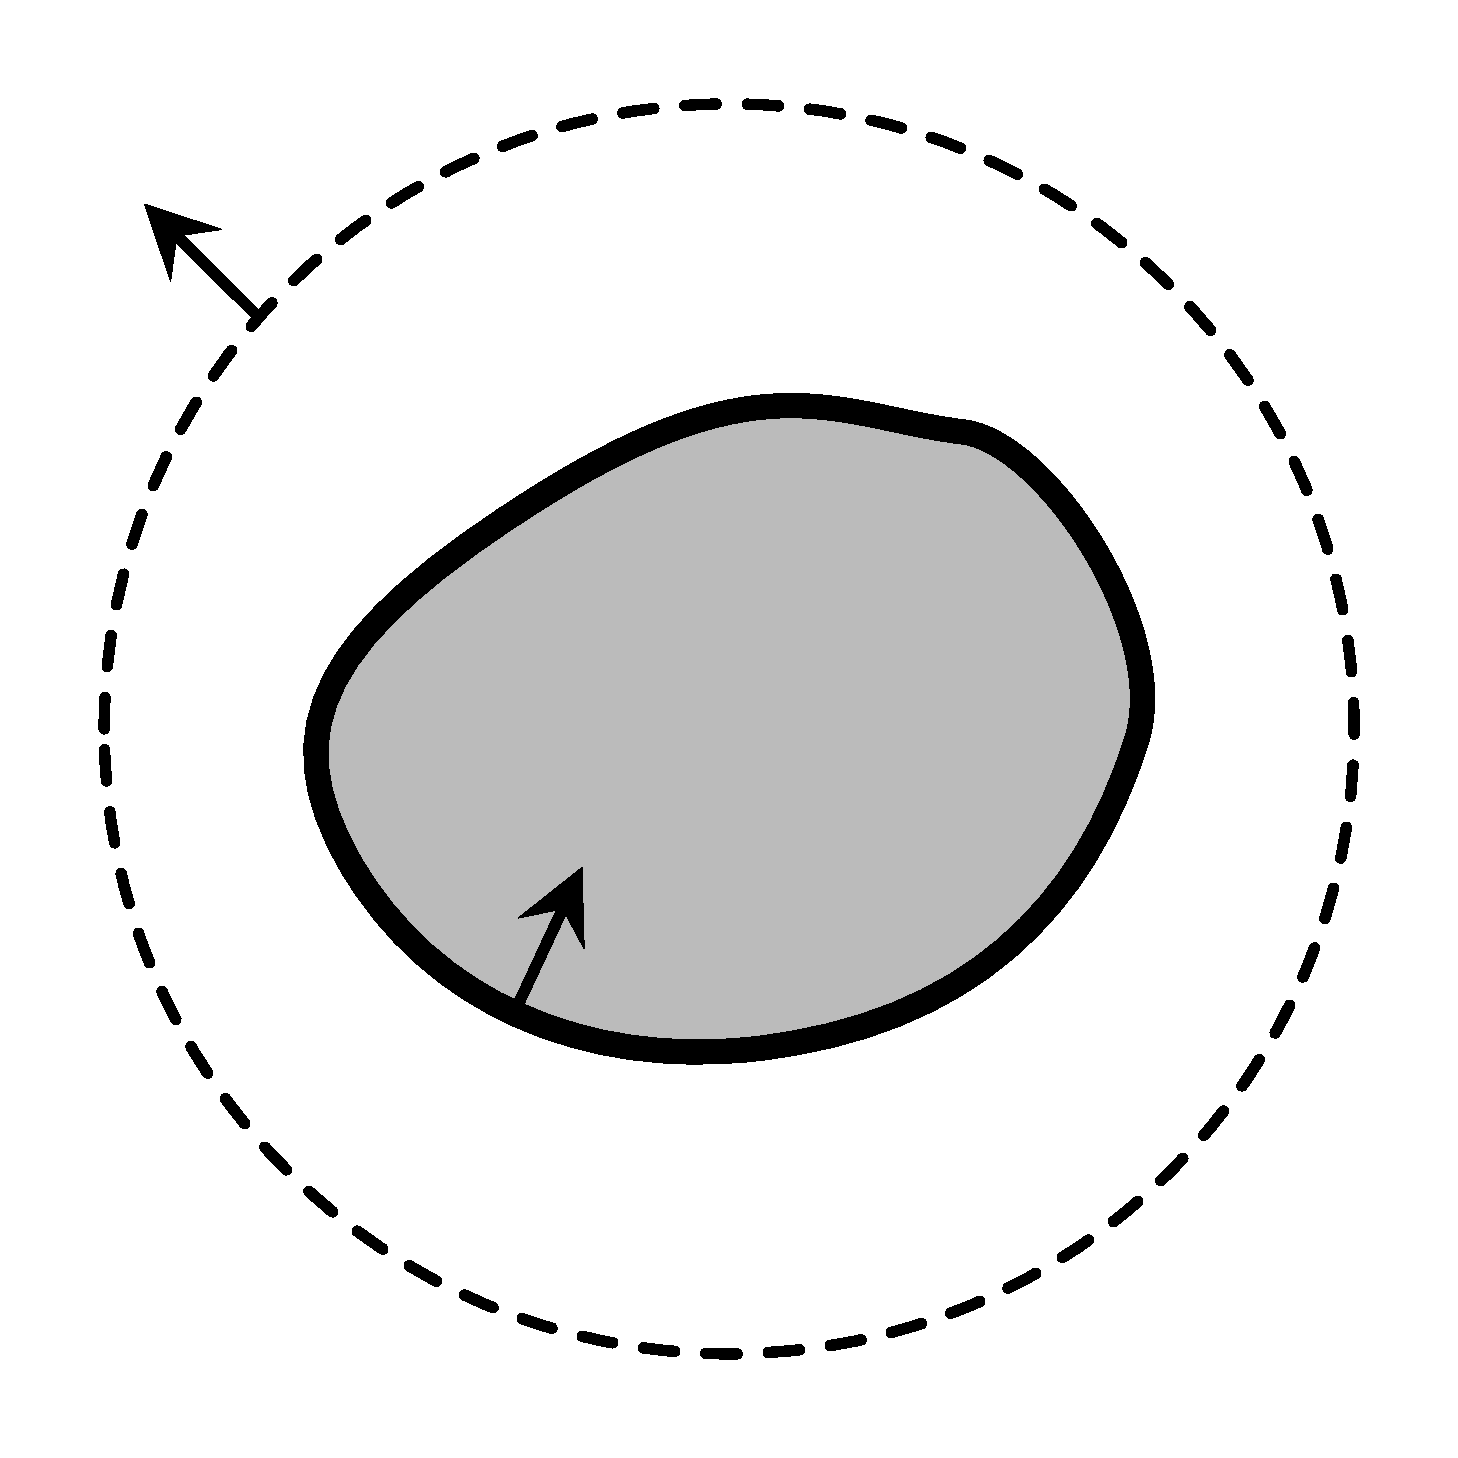
\includegraphics[width=.6\textwidth]{Images/BoundaryIntergral.pdf}};
    \begin{scope}[x={(image.south east)},y={(image.north west)}]
    \begin{scope}[x={(image.south east)},y={(image.north west)}]
        \node at (0.5,0.5) {\Huge $D$};
        \node at (0.41,0.8) {\Huge $S$};
        \node at (0.44,0.39) {\Huge $\bm{n}$};
        \node at (0.15,0.885) {\Huge $\bm{n}$};
    \end{scope}
    \end{scope}
\end{tikzpicture}}
    \caption{A schematic diagram of the volume used in the derivation of the boundary integral for Stokes flow.}
    \label{fig:SystematicDiagram}
\end{figure}

Suppose we now let $S$ be the volume between the solid body $D$ and a sphere with a radius such that all of $D$ is contained within as seen in \cref{fig:SystematicDiagram}. Denoting $\partial S$ to be the surface of $S$, note that $\partial S$ is both the surface of the sphere and the surface of the solid body $\partial D$. Integrating the above equation \cref{eq:reciprocalrelation} over the volume $S$ then we get that
\begin{equation*}
\begin{aligned}
      &\iiint_{S} \left[\frac{1}{8\pi\mu}\frac{\partial}{\partial x_k}(S^\epsilon_{ij}\left(\bm{x}, \bm{y}\right)\sigma_{ik}\left(\bm{x}, \bm{y}\right) - \mu u_i(\bm{x}) T^\epsilon_{ijk}\left(\bm{x}, \bm{y}\right))\right] dV(\bm{x}) \\
      &= \iiint_{S} u_j(\bm{x})\phi_\epsilon(\bm{x}-\bm{y}) dV(\bm{x}).
\end{aligned}
\end{equation*}
Using the divergence theorem on the left-hand side of the equation it is found that
\begin{equation*}
  \frac{1}{8\pi\mu}\iint_{\partial S} \left[S^\epsilon_{ij}\left(\bm{x}, \bm{y}\right)\sigma_{ik}\left(\bm{x}, \bm{y}\right) - \mu u_i(\bm{x}) T^\epsilon_{ijk}\left(\bm{x}, \bm{y}\right)\right]n_k ds(\bm{x}) = \iiint_{S} u_j\phi_\epsilon(\bm{x}-\bm{y}) dV(\bm{x})
\end{equation*}
where $\bm{n}$ is the outwards facing unit normal vector of $\partial S$. Now considering the limit as the radius of the sphere tends to infinity, the only contributions to the left-hand side come from $\partial D$. We will introduce the traction on the surface of the sphere as $g_{i} = -\sigma_{ik}n_k$ (as the unit normal points into $D$) and obtain
\begin{equation}
\begin{aligned}
    \label{eq:BIE3}
    &\frac{1}{8\pi\mu}\iint_{\partial D} S^\epsilon_{ij}\left(\bm{x}, \bm{y}\right)g_i(\bm{x}) ds(\bm{x}) - \frac{1}{8\pi}\iint_{\partial D} u_i(\bm{x}) T^\epsilon_{ijk}\left(\bm{x}, \bm{y}\right)n_k(\bm{x}) ds(\bm{x}) \\
    &= \iiint_{S} u_j(\bm{x})\phi_\epsilon(\bm{x}-\bm{y}) dV(\bm{x})
\end{aligned}
\end{equation}

Considering the fluid inside of the solid body $D$ we realise that the velocity must satisfy the zero-deformation condition
\begin{equation*}
  \frac{\partial u_i}{\partial k} + \frac{\partial u_k}{\partial i} = 0
\end{equation*}
This must mean that the pressure is constant inside of $D$ and reduces the stress to $\sigma_{ik} = -p\delta_{ik}$ inside of $D$ and as such for each $j=1,2,3$
\begin{equation*}
  \iiint_{D} \frac{\partial}{\partial x_k}\left[S^\epsilon_{ij}\left(\bm{x}, \bm{y}\right)\sigma_{ik}\left(\bm{x}, \bm{y}\right)\right]dV(\bm{x}) = -p\iiint_{D} \frac{\partial}{\partial x_k}\left[S^\epsilon_{kj}\left(\bm{x}, \bm{y}\right)\right]dV(\bm{x}) = 0
\end{equation*}
from the incompressibility condition \cref{eq:regcondition2}. Integrating \cref{eq:reciprocalrelation} over the volume $D$ instead of $S$ and using the above integral, it is found that given $p \neq 0$
\begin{equation}
\begin{aligned}
    \label{eq:BIE4}
    -\frac{1}{8\pi}\iiint_{D} \frac{\partial}{\partial x_k}\left(u_i(\bm{x})T^\epsilon_{ijk}\left(\bm{x}, \bm{y}\right) \right) dV(\bm{x}) &= \frac{1}{8\pi}\iint_{\partial D} u_i(\bm{x})T^\epsilon_{ijk}\left(\bm{x}, \bm{y}\right)n_k(\bm{x}) ds(\bm{x})\\
    &= \iiint_D u_j(\bm{x}) \phi^\epsilon(\bm{x}-\bm{y}) dV(\bm{x}).
\end{aligned}
\end{equation}

The divergence theorem is again used to convert the volume integral to a surface integral with $n_k$ being the unit normal pointing into $D$. Observing that the sum over \cref{eq:BIE3,eq:BIE4} will be the integral over all space $\mathbb{R}^{3}$ and, using the fact that the velocity is continuous on the boundary $\partial D$ the final boundary integral equation is determined to be
\begin{equation}
  \label{eq:BIE5}
    \iiint_{\mathbb{R}^{3}} u_{j}(\bm{x}) \phi^{\epsilon}\left(\bm{x}-\bm{y}\right) d V(\bm{x})=-\frac{1}{8 \pi \mu} \iint_{\partial D} S_{i j}^{\epsilon}\left(\bm{x}, \bm{y}\right) g_{i}(\bm{x}) d s(\bm{x}).
\end{equation}
As the traction $\bm{g}$ denotes the traction exerted by the fluid on the body it must have the opposite sign to the stokeslet traction $\bm{f}$ and as such $\bm{f} = -\bm{g}$ where $\bm{f}$ denotes the force per unit area acting on the fluid. To use \cref{eq:BIE5} we need to have an explicit equation for $\bm{u}(\bm{x})$, By taking the approximation that $\int_{\mathbb{R}^{3}} u_{j}(\bm{x}) \phi^{\epsilon}\left(\bm{x}-\bm{y}\right) d V(\bm{x}) \approx u_j(\bm{y})$. By taking the approximation as exact \cref{eq:BIE5} can be written as
\begin{equation}
    u_j(\bm{y}) = \frac{1}{8 \pi \mu} \iint_{\partial D} S_{i j}^{\epsilon}\left(\bm{x}, \bm{y}\right) f_{i}(\bm{x}) d s(\bm{x}).
\end{equation}
By using the fact that $S_{i j}^{\epsilon}\left(\bm{x}, \bm{y}\right) = S_{j i}^{\epsilon}\left(\bm{y}, \bm{x}\right)$ \cref{eq:BIE5} can be written as 
\begin{equation}
  \label{eq:BIE}
    u(\bm{x})_i=\frac{1}{8 \pi \mu} \iint_{\partial D} S_{i j}^{\epsilon}\left(\bm{x}, \bm{y}\right) f_{j}(\bm{y}) d s(\bm{y}).
\end{equation}
The analysis of this error for our particular cutoff function can be seen in \cite{Cortez2005} and is found to be of order $\mathcal{O}(\epsilon)$ close to the boundary and $\mathcal{O}(\epsilon^2)$ away from the boundary.

The analytical computation of \cref{eq:BIE} is possible for certain cases allowing for the computation of the fluid velocity given prescribed body forces on the fluid \cite{Walker2020AFilaments,Zhao2021RegularizedFlow,Ohm2021RemarksTheory,Zhao2019}, however, they are often hard or impossible to do by hand. As such we consider the numerical integration of such problems, by approximating the boundary integral equation with a quadrature rule a formula for the velocity of the fluid at a point $\bm{y}$ can be found. By considering the the integral on the right-hand side of \cref{eq:BIE} as the sum over $N$ stokeslets located on the surface of $D$ the velocity can be approxiamted as
\begin{equation}
\label{eq:Stokesletsum}
    u_{i}\left(\bm{x}\right)=\frac{1}{8 \pi \mu} \sum_{n=1}^{N} \sum_{i=1}^{3} S_{i j}^{\epsilon}\left(\bm{x}, {\bm{y}}_{n}\right) {f}_{j}({\bm{y}}_{n}) A_{n}
\end{equation}
where ${f}_{i}({\bm{y}}_n)$ is the $i$th component of the force on the fluid at the point ${\bm{y}}_n$ and $A_n$ combines both the corresponding quadrature weight of the $n$th stokeslet and surface metric.

The discretisation of the integral in \cref{eq:BIE} introduced a discretisation error of $\mathcal{O}(h)$ where $h$ is the average spacing between quadrature points and also a quadrature error which is also dependent on $\epsilon$. Analysis done by Cortez, Fauci and Medovikov \cite{Cortez2005} estimated the quadrature error introduced by this method to be $\mathcal{O}(h^2\epsilon^{-3})$ although more recent analysis by Gallagher, Choudhuri and Smith \cite{Gallagher2019SharpEquation} refined this estimate to $\mathcal{O}(h^2\epsilon^{-1}) + \mathcal{O}(P\epsilon^{-1/P} h^{1-P})$ for any integer $P>3$. The $\mathcal{O}(h^2\epsilon^{-1})$ regularisation term provides the motivation for most of the subsequent work done in this paper as for a fixed epsilon, reducing the regularisation error requires a reduction in $h$ which increases the number of quadrature points and as such the overall complexity of the numerical problem. 

\subsection{Matrix formulation} \label{subsec:MatrixForm}
The computation of \cref{eq:Stokesletsum} for a set of collocation points $\{\bm{x}_m\}$  for $m = 1,...,M$ can be viewed as the product of a dense $3M \times 3N$ matrix with a $3N \times 1$ column vector where $M$ is the number of collocation points and $N$ the number of stokeslet points. By taking the Nyström \cite{Nystrom1930UberRandwertaufgaben} discretisation where $\{\bm{x}_m\} = \{\bm{y}_n\}$ the stokeslet matrix therefore becomes a $3N \times 3N$ matrix where the velocity can be calculated from a set of prescribed traction's $\{\bm{F}(\bm{x}_n)\}$. 
\begin{equation}
\label{eq:Nystrom}
    u_{i}\left(\bm{x}_m\right)=\frac{1}{8 \pi \mu} \sum_{n=1}^{N} \sum_{i=1}^{3} S_{i j}^{\epsilon}\left(\bm{x}_m, {\bm{x}}_{n}\right) {F}_{j}({\bm{x}}_{n})
\end{equation}
where $n=1,\dots,N$, $m=1,\dots,N$ and $j=1,2,3$. The computation of this matrix-vector product can be written as 
\begin{equation}
\label{eq:matrixvectorproduct}
    \underline{U} = A \underline{F}
\end{equation}
where $\underline{U}$ is a $3N \times 1$ column vector, $A$ is a $3N \times 3N$ matrix and $\underline{F}$ is a $3N \times 1$. We will make the choice to assemble to left hand side of \cref{eq:matrixvectorproduct} as
\small
\begin{equation*}
    \underline{U} = [u_1({\bm{x}}_{1}), \; u_2({\bm{x}}_{1}), \; u_3({\bm{x}}_{1}), \; u_1({\bm{x}}_{2}), \; u_2({\bm{x}}_{2}), \; u_3({\bm{x}}_{2}), \; \dots \; u_1({\bm{x}}_{M}), \; u_2({\bm{x}}_{M}), \; u_3({\bm{x}}_{N})]^{T}u
\end{equation*}
\normalsize
and the vector $\bm{F}$ as
\small
\begin{equation*}
    \underline{F} = [{f}_{1}({\bm{x}}_{1})A_1, \; {f}_{2}({\bm{x}}_{1})A_1, \; {f}_{3}({\bm{x}}_{1})A_1,\; \dots \; {f}_{1}({\bm{x}}_{N})A_N, \; {f}_{2}({\bm{x}}_{N})A_N, \; f_{3}({\bm{x}}_{N})A_N]^{T}
\end{equation*}
\normalsize
This means the structure of $A$ can be written as
\small
\begin{equation}
\begingroup
\setlength\arraycolsep{0.8pt}
A = \begin{bmatrix}
S^{\epsilon}_{11}(\bm{x}_1,{\bm{x}}_1) & S^{\epsilon}_{12}(\bm{x}_1,{\bm{x}}_1) & S^{\epsilon}_{13}(\bm{x}_1,{\bm{x}}_1) & \dots & S^{\epsilon}_{11}(\bm{x}_N,{\bm{x}}_1) & S^{\epsilon}_{13}(\bm{x}_N,{\bm{x}}_1) & S^{\epsilon}_{13}(\bm{x}_N,{\bm{x}}_1)\\
S^{\epsilon}_{21}(\bm{x}_1,{\bm{x}}_1) & S^{\epsilon}_{22}(\bm{x}_1,{\bm{x}}_1) & S^{\epsilon}_{23}(\bm{x}_1,{\bm{x}}_1) & \dots & S^{\epsilon}_{21}(\bm{x}_N,{\bm{x}}_1) & S^{\epsilon}_{22}(\bm{x}_N,{\bm{x}}_1) & S^{\epsilon}_{23}(\bm{x}_N,{\bm{x}}_1)\\
S^{\epsilon}_{31}(\bm{x}_1,{\bm{x}}_1) & S^{\epsilon}_{32}(\bm{x}_1,{\bm{x}}_1) & S^{\epsilon}_{33}(\bm{x}_1,{\bm{x}}_1) & \dots & S^{\epsilon}_{31}(\bm{x}_N,{\bm{x}}_1) & S^{\epsilon}_{32}(\bm{x}_N,{\bm{x}}_1) & S^{\epsilon}_{33}(\bm{x}_N,{\bm{x}}_1)\\
\vdots & \vdots & \vdots & \ddots & \vdots & \vdots & \vdots \\
S^{\epsilon}_{11}(\bm{x}_1,{\bm{x}}_N) & S^{\epsilon}_{12}(\bm{x}_1,{\bm{x}}_N) & S^{\epsilon}_{13}(\bm{x}_1,{\bm{x}}_N) & \dots & S^{\epsilon}_{11}(\bm{x}_N,{\bm{x}}_N) & S^{\epsilon}_{12}(\bm{x}_N,{\bm{x}}_N) & S^{\epsilon}_{13}(\bm{x}_N,{\bm{x}}_N)  \\
S^{\epsilon}_{21}(\bm{x}_1,{\bm{x}}_N) & S^{\epsilon}_{22}(\bm{x}_1,{\bm{x}}_N) & S^{\epsilon}_{23}(\bm{x}_1,{\bm{x}}_N) & \dots & S^{\epsilon}_{21}(\bm{x}_N,{\bm{x}}_N) & S^{\epsilon}_{22}(\bm{x}_N,{\bm{x}}_N) & S^{\epsilon}_{23}(\bm{x}_N,{\bm{x}}_N) \\
S^{\epsilon}_{31}(\bm{x}_1,{\bm{x}}_N) & S^{\epsilon}_{32}(\bm{x}_1,{\bm{x}}_N) & S^{\epsilon}_{33}(\bm{x}_1,{\bm{x}}_N) & \dots & S^{\epsilon}_{31}(\bm{x}_N,{\bm{x}}_N) & S^{\epsilon}_{32}(\bm{x}_N,{\bm{x}}_N) & S^{\epsilon}_{33}(\bm{x}_N,{\bm{x}}_N) \\
\end{bmatrix}
\endgroup
\label{eq:StokeletMatrix}
\end{equation}
\normalsize
We do note that this choice in the structure of $\underline{U}$ and $\underline{F}$ is not unique and other literature may use different arrangements. The computation of matrix vector product requires $9N^2$ function evaluations to assemble to stokeslet matrix followed by $\mathcal{O}(N^2)$ operations to compute the vector product. This becomes prohibitive in both computation time and memory usage when considering systems of large $N$ and for later comparison with other algorithms we will refer to this method of computation as the direct product.

\subsection{Resistance Problem} \label{sec:resistance}
A common problem to solve in Stokes flow is the resistance problem, where the force distribution, and hence total force and moment, on a body is calculated from a prescribed rigid body motion. By taking the Nyström discretisation
and prescribing velocities at each point $\{\bm{x}_m\}$ a system of $3M$ equations with $3N$ unknowns $F_j(\bm{y}_n) := f_j(\bm{y}_n)A_n$ is formed. For each of the rigid body motion modes, unit velocity translation along each axis and unit angular velocity rotation about each axis, are calculated we can form the grand resistance matrix $\mathcal{R}$ \cite{Pozrikidis1992BoundaryFlow}. By the linearity of the Stokes equation, $\mathcal{R}$ relates the force $\mathbf{F}$ and moment $\mathbf{M}$ to the velocity $\mathbf{U}$ and angular velocity $\mathbf{\Omega}$ for any rigid body motion. 
\begin{equation}
\arraycolsep=1pt\def\arraystretch{1.2}
\left(
\begin{array}{c}
\boldsymbol{F} \\
\boldsymbol{M}
\end{array}\right)=\underbrace{\left(\begin{array}{cc}
A_{F U} & A_{F \Omega} \\
A_{M U} & A_{M \Omega}
\end{array}\right)}_{\mathcal{R}}\left(\begin{array}{c}
\boldsymbol{U} \\
\boldsymbol{\Omega}
\end{array}\right) .
\label{eq:GrandResistance}
\end{equation}
 For example, Stokes' Law gives us that the grand resistance matrix for a sphere of radius $r$ centred at the origin is
 \begin{equation}
\arraycolsep=1pt\def\arraystretch{1.2}
\mathcal{R}=\left(\begin{array}{cc}
6\pi\mu r I & 0 \\
0 & 8\pi\mu r^3 I
\end{array}\right)
\label{eq:sphereres}
\end{equation}
where $I$ is the $3\times 3$ identity matrix and $0$ is a $3\times 3$ matrix of zeros.

The most common method for solving the resistance problem is to generate the full stokeslet matrix and solve the subsequent linear system $\underline{U} = A\underline{F}$ for $\underline{F}$, this problem can either be solved through the inversion of the matrix $A$ or, in our implementation, the use of MATLAB's \textit{mldivide} ($\backslash$) function which both take $\mathcal{O}(N^3)$ operations to compute the solution force dense systems. For the Nyström discretisation we have an regularisation error term of $\mathcal{O}(h^2\epsilon^{-1})+\mathcal{O}(\epsilon)$ so in order to keep a fixed $\epsilon$ and still reduced the error, the quadrature spacing needs to be decreased and as such the $N$ grows. As such for larger systems the use of mldivide becomes too computationally costly, either from time or memory usage, the solution can be solved using the Generalized Minimal RESidual (GMRES) method (See \cref{appendix:GMRES}) \cite{Saad1986GMRES:Systems,Elman2005FiniteDynamics}. GMRES can perform the inverse in at worst $\mathcal{O}(N)$ iterations (with each iteration requiring $\mathcal{O}(N^2)$ operations) however will often converge to a solution with a small relative residual error in significantly fewer iterations, particularly when an appropriate preconditioner is used. 